\section{Use Case : B�timent intelligent}

Ce "use case" est celui du d�ploiement d'objets connect�s dans
un b�timent que l'on voudrait rendre intelligent..

\subsection{Le besoin}
L'UCA veut conna�tre les temp�ratures des salles de TOUS ses
b�timents afin de savoir si le contrat de "temp�rature constante"
qu'elle a souscrit avec une soci�t� est respect�.

\medskip
Elle envisage donc de s'�quiper d'objets communicants pour surveiller
cela.

Il y aura un poste de surveillance � l'accueil de chaque b�timent.

\medskip
\begin{dinglist}{227}
\item La valeur de la "temp�rature constante" contractuelle est
  fonction des salles.
\end{dinglist}

\medskip
Ceci �tant dit, vous pouvez augmenter le cahier des charges :

\medskip
Aller plus loin en int�grant une gestion pilot�e
des radiateurs en fonction de la temp�rature relev�e.

\medskip Il y aura aussi un mode jour-nuit (crit�re horaire) qui
adaptera le seuil des salles, d�s lors que la salle est inoccup�e
(c'est le crit�re de luminosit� qui indique cela).

\medskip
Les capteurs de temp�ratures peuvent aussi servir � g�rer les risques
d'incendies, il faut alors pr�venir le centre technique de l'UCA
\textbf{et} les pompiers !

\medskip
Puisqu'on parle du centre technique, les capteurs peuvent �tre
d�faillants, c'est le centre technique et l'accueil du b�timent qui
doivent g�rer cela. 

\medskip
Les objets peuvent aussi d�tecter les salles rest�es allum�es, \ldots


\subsection{Les pistes pour un tel sujet \ldots}

Bien s�r vous utiliserez les capteurs d�j� manipul�s mais au del�
\ldots

\medskip
Toujours pareil \ldots que des propositions !

Sur un tel sujet, le dashboard et la repr�sentation du terrain, avec le
positionnement / la repr�sentation / la d�signation des capteurs peut
�tre un plus \ldots

\begin{center}
  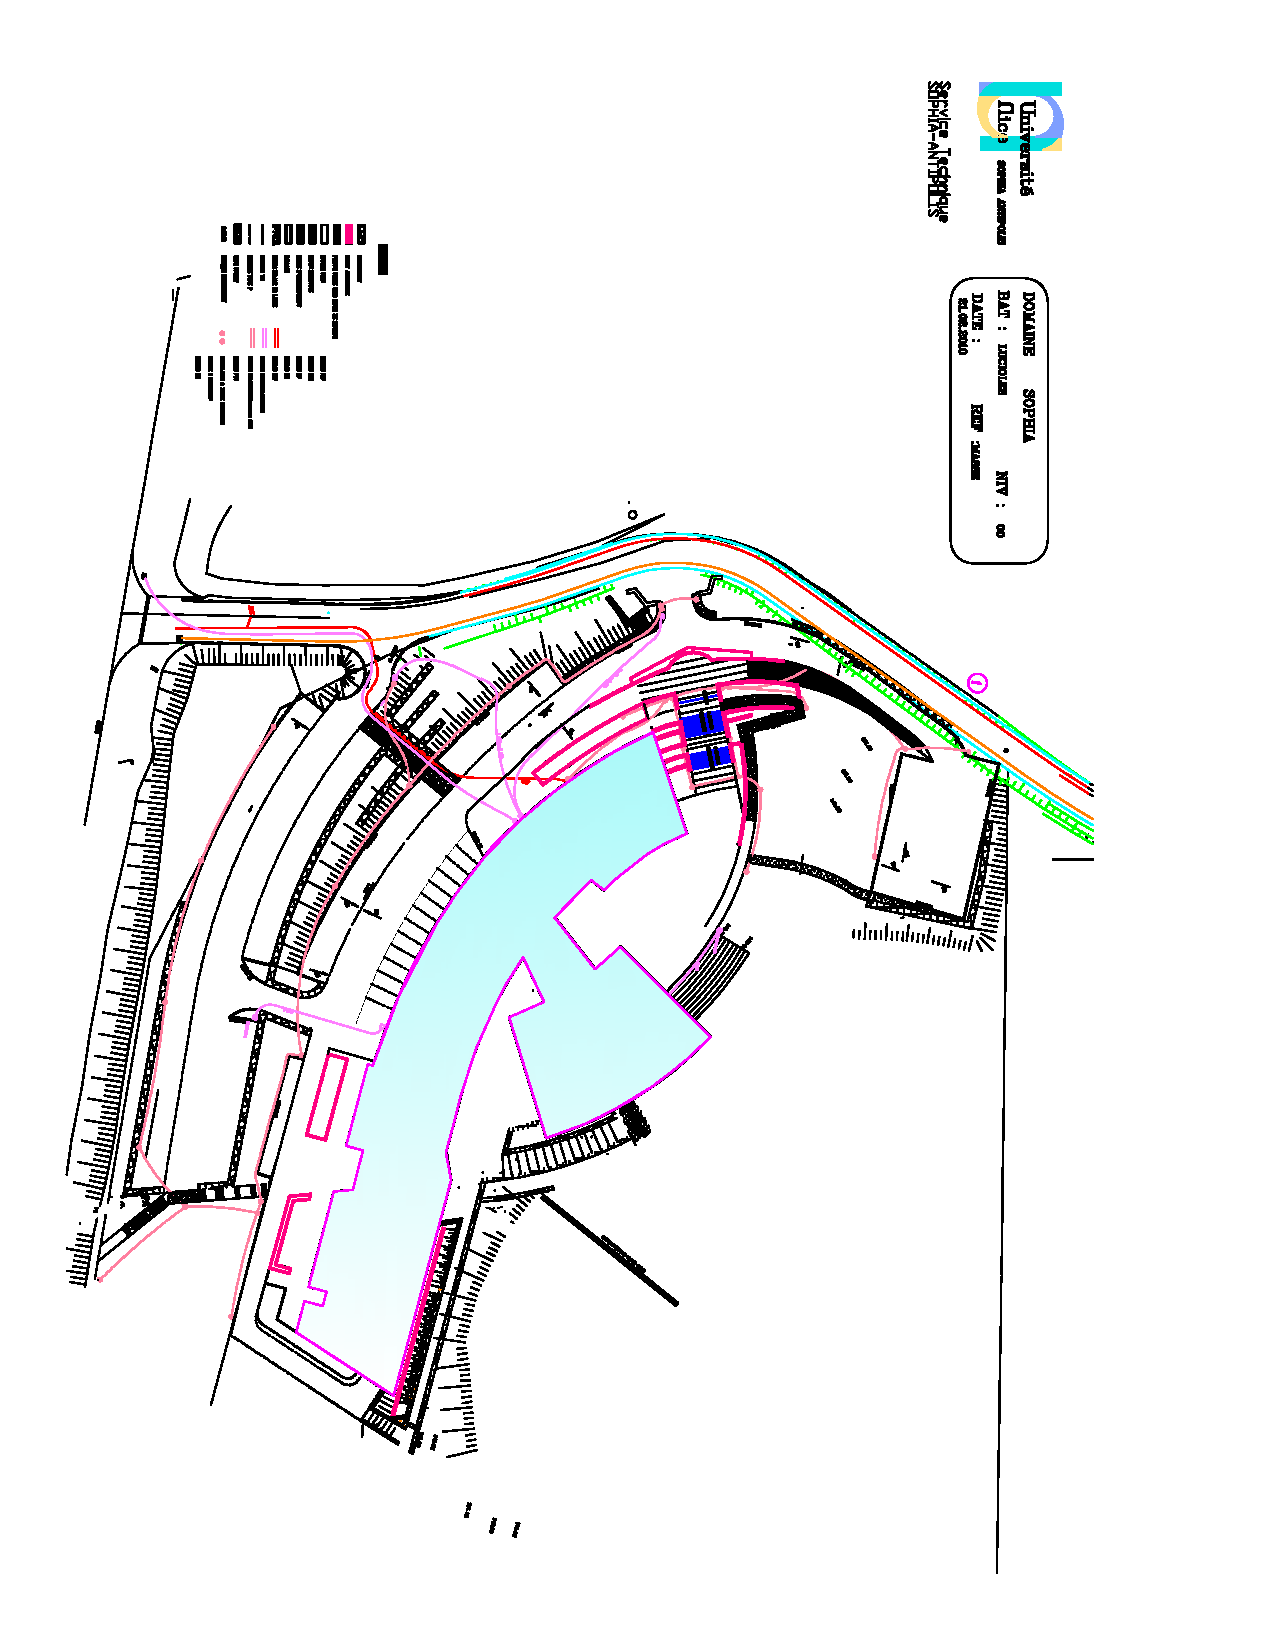
\includegraphics[scale=0.6, angle=90]{PlansLucioles/EsMasseBIS-MASSE}
\end{center}

Est ce que l'on peut faire quelque chose qui soit aussi
dynamique/�volutif ?!


\endinput